\documentclass[tikz,border=10pt]{standalone}
\usepackage[T1]{fontenc}
\usetikzlibrary{backgrounds}
\begin{document}
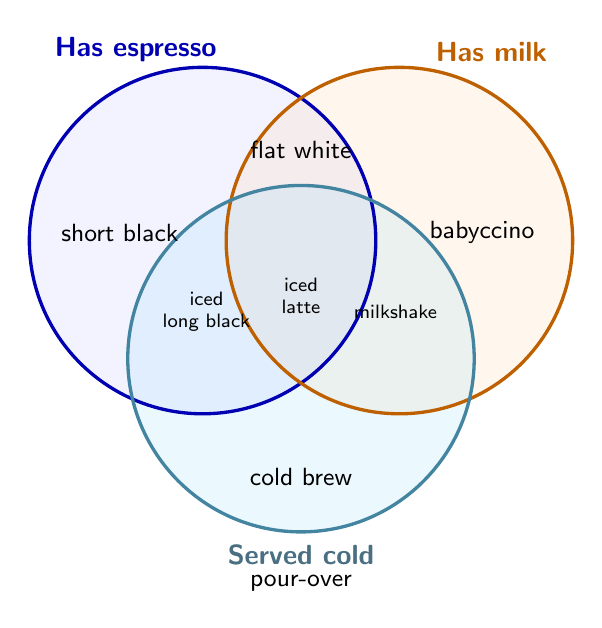
\begin{tikzpicture}[font=\sffamily]
  % Three sets: espresso, milk, and served cold.
  \begin{scope}[on background layer]
    \fill[blue!45, fill opacity=.10] (-1.25,.55) circle (2.2);
    \fill[orange!65, fill opacity=.10] (1.25,.55) circle (2.2);
    \fill[cyan!65, fill opacity=.12] (0,-.95) circle (2.2);
  \end{scope}
  \draw[blue!70!black, line width=1.2pt] (-1.25,.55) circle (2.2);
  \draw[orange!75!black, line width=1.2pt] (1.25,.55) circle (2.2);
  \draw[cyan!60!black, line width=1.2pt] (0,-.95) circle (2.2);

  % Set labels
  \node[blue!70!black, font=\sffamily\bfseries, anchor=south west] at (-3.25,2.7) {Has espresso};
  \node[orange!75!black, font=\sffamily\bfseries, anchor=south east] at (3.25,2.7) {Has milk};
  \node[cyan!45!black, font=\sffamily\bfseries, anchor=north] at (0,-3.2) {Served cold};

  % Drinks in their respective regions
  \node[align=center, font=\sffamily\small] at (-2.3,.65) {short black};
  \node[align=center, font=\sffamily\small] at (2.3,.65) {babyccino};
  \node[align=center, font=\sffamily\small] at (0,1.7) {flat white};
  \node[align=center, font=\sffamily\scriptsize] at (-1.2,-.35) {iced\\long black};
  \node[align=center, font=\sffamily\scriptsize] at (1.2,-.35) {milkshake};
  \node[align=center, font=\sffamily\scriptsize] at (0,-.15) {iced\\latte};
  \node[align=center, font=\sffamily\small] at (0,-2.45) {cold brew};
  \node[align=center, font=\sffamily\small] at (0,-3.8) {pour-over};
\end{tikzpicture}
\end{document}
